\problemname{Brickor}

Karin har hittat på ett ensamspel som spelas med Othello-brickor, vilka är
svarta på ena sidan och vita på andra sidan. Hon lägger ut en rad med
brickor, som var och en kan vara svart eller vit. Målet är att få alla brickor att ha den vita sidan uppåt.

Ett ``drag'' är att ``plocka ut'' ett intilliggande par av brickor
någonstans ur sekvensen, vända på dem (vit blir svart, svart blir
vit), och lägga tillbaka dem antingen i början av raden eller i slutet av
raden, utan att ändra parets inbördes ordning.

Skriv ett program som, givet den ursprungliga raden av brickor, 
skriver ut det minsta antalet drag som behövs för
att göra alla brickor vita.

\begin{center}
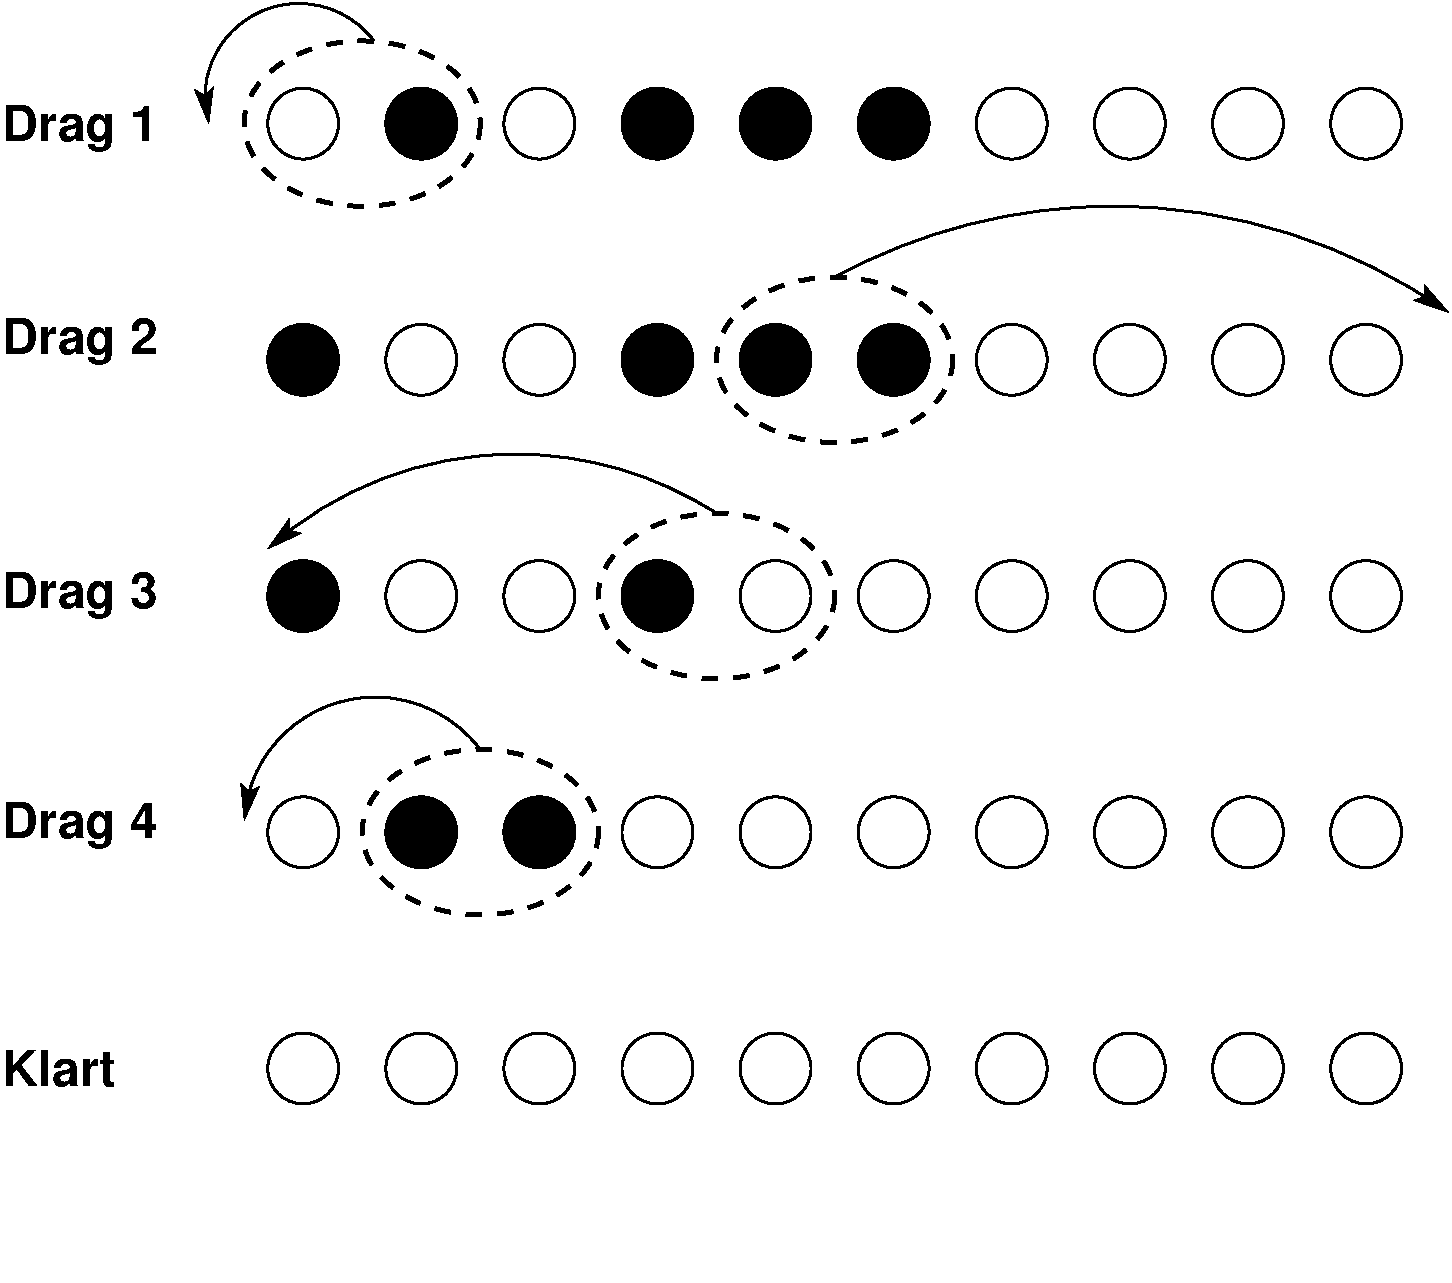
\includegraphics[width=12cm]{brickorbild.pdf}\\
{\em En möjlig dragsekvens i exempel 2}
\end{center}

\section*{Indata}

Indata består av en sträng med enbart bokstäverna \texttt S och \texttt V.
Strängen är mellan 3 och 15 tecken lång.

\section*{Utdata}

Skriv ut ett enda tal: det minsta antalet drag som behövs för
att göra alla brickor vita. För givna testdata kommer det alltid vara
möjligt att nå målet.

\section*{Poängsättning}
För testfall värda $60$ poäng är strängens längd högst 10, och svaret är högst 6.\\
För testfall värda $40$ poäng gäller inga speciella begränsningar.
